% !TEX root = twibop2.tex

\chapter{Mathematics of Randomness}
\epigraph{This doctrine, combining the accuracy of mathematical proofs
  and the uncertainty of chance occasions and making peace between
  these seemingly contradictory elements has a full right to contend
  for the title of the mathematics of the random.}{Blaise Pascal}

\section{Probability} 

\txthead{Classical definition of probability.} When
we toss a coin, we do not know which will land face up, heads or
tails. However, there is something we do know. We know that the
chances of both heads and tails are equal. We also know that the
chances of any of the faces of a die landing face up are equal. That
the chances are equal in both examples is due to \redem{symmetry}. Both the
coin and the die are symmetrical. When two or more events have equal
chances of occurring, we call them equally possible outcomes. Heads or
tails are \redem{equally possible} outcomes. Suppose we are interested in a
certain result while throwing a die, for instance, a face with a
number of dots exactly divisible by three. Let us call outcomes
satisfying such a requirement \redem{favourable}. There are two favourable
outcomes in our example, namely, a three or a six. Now let us call
outcomes \redem{exclusive} if the appearance of one in single trial makes it
impossible for the others to appear at the same trial. A die cannot
land with several faces up, so they are exclusive outcomes.  

We can now formulate the classical definition of probability: 
\begin{mybox}{}
The probability of an event is the ratio of the number of favourable outcomes to the total number of equally possible exclusive outcomes.
\end{mybox}

Suppose $P_{A}$ is the probability of an even $A$, $m_{A}$ is the
number of favourable outcomes, and $n$ the total number of equally
possible and exclusive outcomes. According to the classical definition
of probability 
\begin{equation}%
P_{A} = \dfrac{m_{A}}{n}.
\label{eq-1.1}
\end{equation}
If $m_{A} =n$, then $P_{A}= 1$ and the event $A$ is a \redem{certain}
event (it always occurs in every outcome). If $m_{A} =0 $, then $P_{A}
=0$, and the event $A$ is an \redem{impossible} event (it never
occurs). The probability of a \redem{random} event lies between $0$ and
$1$. 

Let an event $A$ be throwing a die and getting a number exactly
divisible by three. Here $m_{A} = 2$ and so the probability of the
event is 1/3, because $n=6$. Consider one more example. We have a
bag with 15 identical but differently coloured balls (seven white, two green, and six
red). You draw a ball at random. What is the probability of drawing
a white (red or green) ball? Drawing a white ball can be regarded as an
event $A$, drawing a red ball is an event $B$, and drawing a green ball is an event $C$. The number of favourable outcomes of drawing a ball of
a certain colour equals the number of balls of this colour, i. e., $m_{A} = 7$, $m_{B} = 6$, and $m_{C} = 2$. Using (\ref{eq-1.1}) and given $n = 15$, we can find the
probabilities:
\begin{equation*}
P_{A} = \dfrac{m_{A}}{n} = \dfrac{7}{15}, \quad P_{B} =
\dfrac{m_{B}}{n} = \dfrac{2}{15}, \quad P_{C} = \dfrac{m_{C}}{n} = \dfrac{2}{15}. 
\end{equation*}

\txthead{Addition and multiplication of probabilities.} What is the probability that a randomly drawn ball will be either red or green? The number of favourable outcomes is $m_{B} + m_{C} = 6 + 2 = 8$, and therefore the probability will be
\begin{equation*}%
P_{B+C} = \frac{m_{B}+m_{C}}{n} = \frac{8}{15}.
\end{equation*} 
We see that $ P_{B+C} = P_{B} + P_{C} $. The probability of drawing either a red or a green ball is the sum of two probabilities: the probability of drawing a red ball and that of drawing a green ball. The probability of drawing a ball which is either red or green or white is the sum of three probabilities, $P_{A} + P_{B} + P_{C}$. It is equal to unity $(7/15 + 2/5 + 2/15 = 1)$. This stands to reason because the event in question will always occur.

The rule for adding probabilities can be formulated as follows: 
\begin{mybox}{}
The probability of one event of several exclusive events occurring is the sum of the probabilities of each separate event.
\end{mybox}

\newcolumntype{g}{>{\columncolor{LightYellow}}c}
%\begin{table}[ht]

\begin{figure}
\begin{footnotesize}
\centering
\setlength\arrayrulewidth{1.25pt}\arrayrulecolor{Tomato}
\begin{tabular}{gggggg}
\hline
%&col1 &col2 &col3 &col4 & col5 &col6 &col7\\
%\hline
% row1& \ra & \ra & \ra & \ra & \ra & \ra & \ra \\
% row2& \ra & \ra & \ra & \ra & \ra & \ra & \ra \\
% row3& \ra & \ra & \ra & \ra & \ra & \ra & \ra \\
% row4& \ra & \ra & \ra & \ra & \ra & \ra & \ra \\
% row5& \ra & \ra & \ra & \ra & \ra & \ra & \ra \\
% row6& \ra & \ra & \ra & \ra & \ra & \ra & \ra \\
\cellcolor[gray]{0.8}(1,1) & (2,1) & (3,1) & (4,1) & (5,1) & (6,1) \\
(1,2) & \cellcolor[gray]{0.8}(2,2) & (3,2) & (4,2) & (5,2) & (6,2) \\
(1,3) & (2,3) & \cellcolor[gray]{0.8}(3,3) & (4,3) & (5,3) & (6,3) \\
(1,4) & (2,4) & (3,4) & \cellcolor[gray]{0.8}(4,4) & (5,4) & (6,4) \\
(1,5) & (2,5) & (3,5) & (4,5) & \cellcolor[gray]{0.8}(5,5) & (6,5) \\
(1,6) & (2,6) & (3,6) & (4,6) & (5,6) & \cellcolor[gray]{0.8}(6,6) \\
\hline
\end{tabular}
\caption{Possible outcomes of rolling a die.\label{die-table}}
\end{footnotesize}
%fig 1.1
\end{figure}

Suppose that two dice are thrown. What is the probability of getting
two fours at the same time? The total number of equally possible
exclusive outcomes is $n = 6 \times 6 = 36$. Each one is listed in \figr{die-table}, where the left figure in the parentheses is the number on one die, and the right figure is the number on the other. There is only one favourable outcome, and it is indicated in \figr{die-table} as (4,4). Hence, the probability of the event is 1/36. This probability is the product of two probabilities: the probability of a four appearing on one die and that of a four on
the other i.e. 
\begin{equation*}%
P_{44} = P_{4} \times P_{4} = \frac{1}{6} \times \frac{1}{6} = \frac{1}{36}.
\end{equation*}

The rule for multiplication of probabilities can be formulated as
follows:
\begin{mybox}{}
The probability of several events occurring simultaneously equals the product of the probabilities of each separate event.
\end{mybox}
By the was, it is not necessary for the events to be simultaneous. Instead of throwing two dice at the same time, we could throw a
 single die twice. The probability of getting two fours at the same
 time when two dice are thrown is the same as the probability of
 getting two fours when one die is thrown twice.

 \begin{figure}[t]
 \centering
 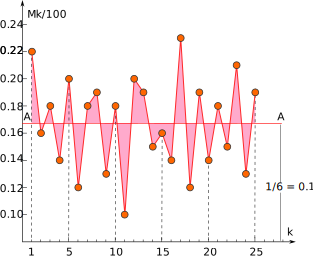
\includegraphics[width=0.9\textwidth]{figures/die-graph.pdf}
\caption{Outcomes of rolling a dice many times.\label{die-graph}}
%fig 1.2
 \end{figure}
 
 
In many cases both rules (addition and multiplication of
probabilities) are used jointly to calculate the probability of an
event. Suppose we are interested in the probability $P$ of the \redem{same} number coming up on two dice. Since it is only essential that the numbers be equal, we can apply the rule for adding probabilities,
\begin{equation*}
P = P_{11} + P_{22} + P_{33} + P_{44} + P_{55} + P_{66}.
\end{equation*}
Each of the probabilities $P_{ii}$ is, in turn, a product $P_{i} \times P_{i}$. \redem{Hence}
\begin{equation*}
P = (P_{1} \times P_{1}) + (P_{2} \times P_{2}) + \ldots + (P_{6}
\times P_{6}) = 6 \left( \dfrac{1}{6} \times \dfrac{1}{6} \right) = \dfrac{1}{6}.
\end{equation*}
This result can be obtained right away from \figr{die-table}, where
the favourable outcomes are shown in the gray, (1,1), (2,2), (3,3),
(4,4), (5,5), and (6,6). The total number of such outcomes is six. Consequently, $P = 6/36 = 1/6$.

\txthead{Frequency and probability.} The classical
definition of probability and the rules for addition and
multiplication of probabilities can be used to calculate the
probability of a random event. However, what is the practical value of
such calculations? For instance, what does it mean in practice that
the probability of getting a four when a die is thrown equals 1/6? Naturally, the assertion does not imply that a four will appear once and only once in any six trials. It is possible that it will appear once, but it is also possible that it will appear two (or more) times, or that it will not appear at all. In order to discover the probability of an event in practice we should perform a large number of trials and calculate how frequently a four appears.


Let us perform several sets of trials, for instance, throwing the die
100 times in each set. Let us designate $M_{1}$ to be the number of
times a four appears in the first set, $M_{2}$ to be the
number of fours in the second set, etc. The ratios
$M_{1}/100, M_{2}/100, M_{3}/100, \ldots{} $ are the frequencies with
which a four appeared in each set. Having performed several sets of
trials, we can see that the frequency of the appearance of a four
\redem{varies from set to set in a random fashion in the vicinity of
  the probability} of the trials, we can see that the frequency of the
appearance of a four \redem{varies} from set to set \redem{in a random
  fashion in the vicinity of the probability} of the given event,
i.e. in the vicinity of 1/6. This is clear from \figr{die-graph}, where the number $k$ of sets of trials is plotted along the abscissa axis and the frequencies with which a four appears along
the axis of ordinates. 

\begin{figure}%[ht]
 \centering
 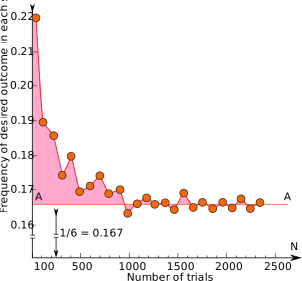
\includegraphics[width=0.9\textwidth]{figures/die-graph2.pdf}
\caption{Frequencies of outcomes of trials of a die as a function of number of trials. Note how the deviation of the frequency of the occurrence of an event from its probability decreases as the number of trials increases.\label{die-graph2}}
 \end{figure}
 
Naturally, if we perform the experiment again,
we will get other values of the frequencies $M_{k}/100$. However, the
pattern of oscillations of the frequencies of the event under
consideration will be stable: the deviations upwards and downwards
from the straight line $AA$, which is associated with the probability
of the event, will balance. Even though the amplitudes of the
deviations will vary from set to set, they will not tend to grow or
decrease. This is a consequence of the \redem{equivalence} of each set
of trials. The number of trials in each set is the same, and the
results obtained in a given set do not depend on the results in any
other set.


 

Let us make an important change in that we gradually increase the
number of trials in each set. Using the results of our previous
experiment, as presented in \figr{die-graph}, let us obtain a new
result by \redem{adding} the value of a set of trials to the result of
the preceding sets. In other words, we calculate the number of fours
in the first 100 trials (in our case, $M_{1} = 22$), then the number of
fours in the first 200 trials $(M_{1} + M_{2} = 22 + 16 = 38)$, the in
the first 300 trials  $(M_{1} + M_{2} +  M_{3}  = 22 + 16 + 18 = 56)$
etc. We then find the frequencies of getting a four in the each new
set: $M_{1}/100 = 0.22$, $(M_{1} + M_{2} )/200 = 0.19$, $(M_{1} +
M_{2} +  M_{3})/300  = 0.187$, etc.  These frequencies are plotted in
\figr{die-graph2} against the number of trials in each set (100,
200, \ldots, 2500). The figure demonstrates a crucial fact: the
deviation of the frequency of the occurrence of an event from its
probability decreases as the number of trials increases. In other
words, 
\begin{mybox}{}
frequency of the occurrence of a random event tends to its probability with increasing number of trials.
\end{mybox}




\txthead{Is it possible to give a definition of probability based on frequency?}
Since the frequency of the occurrence of a random event tends to its
probability as the number of trials increases, we might well ask whether
we can define the probability of an event as the limit of the ratio of the
number of its occurrence to the number of trials as the number of trials
lends to infinity. Suppose $N$ is the number of trials and $M_{A} (N)$ is the
number of occurrence of an event A. We want to know whether we can
define the probability $P_{A}$ of the event $A$ as

\begin{equation}
P_{A} = \lim_{N \rightarrow \infty}  \left[ \frac{M_{A} (N)}{N}
\right].
\label{eq-1.2}
\end{equation}

Richard von Mises (1883-1953), a German mathematician of the early
20th century, believed that equation \eqref{eq-1.2} could be considered
a definition of the probability of a random event, and he called it
the \redem{frequency} definition of probability. Von Mises pointed out
that the classical definition of probability \eqref{eq-1.1}
only ``works'' when there is a \redem{finite} number of \redem{equally}
possible outcomes. For instance, situations involving the throwing of
coins or dice.


However, we often encounter situations without the \redem{symmetry}
that determines whether the outcomes are equally possible. These are
the cases when we cannot apply the classical definition of
probability. Von Mises assumed that then the frequency definition can
be used because it does not require a finite number of equally
possible outcomes and, moreover, does not require any calculation of
probability at all.  A probability using the frequency approach is
determined by experiment rather than being calculated.


However, is it possible to determine the probability of a random event
in practice using \eqref{eq-1.2}? The relationship
presupposes an \redem{infinite} number of identical trials. In
practice, we must stop at a \redem{finite} number of trials, and it is
debatable what number to stop at. Should we stop after a hundred
trials, or is it necessary for there to be a thousand, a million, or a
hundred million? And what is the accuracy of the probability
determined in such a way? There are no answers to these questions.
Bcsides, it is not practicable to provide the same conditions while
performing a very large number of trials, to say nothing of the fact
that the trials may be impossible to repeat.


Consequently, relationship \eqref{eq-1.2} is practically
useless, moreover it is possible to prove (though I shall not do so)
that the limit in \eqref{eq-1.2} \redem{does not} strictly
speaking \redem{exist}. This means that the Von Mises's error was that
he made an unwarranted generalization from a correct proposition: he
concluded that the probability of a random even is the limit of the
frequency of its occurrence when the  number of trials tends to
infinity from the correct observation that the frequency of the
occurrence of a random even approaches its probability as the number
of trials increases. 

\txthead{Geometrical definition of probability.}
Suppose that two people have agreed to meet at a certain place between
nine and ten o'clock. They also agreed that each would wait for a
quarter of an hour and, if the other didn't arrive, would leave. What
is the probability that they meet?  Suppose $x$ is the moment one
person arrives at the appointed place, and $y$ is the moment the other
arrives. Let us consider a point with coordinates $(x, y)$ on a plane
as an outcome of the rendezvous. Every possible outcome is within the
area of a square each side of which corresponds to one hour ( Figure
\ref{prob-meeting}). The outcome is favourable (the two meet) for all
points $(x, y)$ such that $\vert \, x - y \, \vert \le 1/4$. These
points are within the blue part of the square in the \figr{prob-meeting}. 
  
  \begin{figure}[ht]
 \centering
 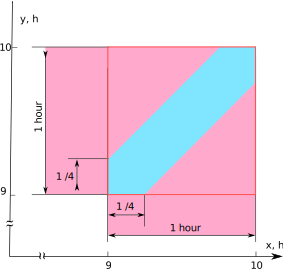
\includegraphics[width=0.9\textwidth]{figures/prob-meeting.pdf}
\caption{Finding the probability using the geometrical method.\label{prob-meeting}}
%fig 1.4
 \end{figure}
  
  All the outcomes are exclusive
and equally possible, and therefore the probability of the rendezvous
equals the ratio of the blue area to the area of the square. This
is reminiscent of the ratio of favourable outcomes to the total number
of equally possible outcomes in the classical definition of
probability. It should be borne in mind that this is a case where the
number of outcomes (both favourable and unfavourable) is
infinite. Therefore, instead of calculating the ratio of the number of
favourable outcomes to the total number of outcomes, it is better to
consider here the ratio of the area containing favourable outcomes to
the total area of the random events.




It is not difficult to use \figr{prob-meeting} and find the
favourable area; it is the difference between the area of the whole
square and the unhatched area, i.e. $1 - \left( 3/4 \right)^2 =
7/16 \, h^{2}$. Dividing $7/16 \, h^{2}$ by $1\, h^{2}$, we find the probability of the rendezvous to be 7/16.

This example illustrates the geometrical definition of probability:
\begin{mybox}{}
The probability of a random event is the ratio of the area favourable for an
event to the total area of events.
\end{mybox}
The geometrical definition of probability is a generalization of the classical definition for the case when the number of equally possible outcomes is infinite.


\txthead{The development of the concept of
    probability.} Although probabilistic notions were used by ancient
Greek philosophers (such as Democritus, Epicurus, and Carus
Lucretius), the theory of probability as a science began in the
mid-$17^{\text{th}}$ century, with the work of the French scientists Blaise
Pascal and Pierre Fermat and the Dutch scientist Christian
Huygens. The classical definition for the probability of a random
event was formulated by the Swiss mathematician Jacob Bernoulli in
\redem{Ars conjectandi} (The Art of Conjectures). The definition was
given its final shape later by Pierre Laplace. The geometrical
definition of probability was first applied in the $18^{\text{th}}$
century. Important contributions to probability theory were made by
the Russian mathematical school in the $19^{\text{th}}$ century (P.L. Chebyshev,
A.A. Markov, and A.M. Lyapunov). 

The extensive employment of probabilistic concepts in physics and technology demonstrated, by the early $20^{\text{th}}$ century, that there was a need for a more refined definition of probability. It was necessary, in particular, in order
to eliminate the reliance of probability on ``common sense''.  An
unsuccessful attempt to give a general definition for the probability
of a random event on the basis of the limit of its frequency of
occurrence was made, as we have seen, by Richard von Mises.  However,
an \redem{axiomatic} approach rather than a frequency one resulted in more
refined definition of probability. The new approach was based on a
set of certain assumptions (axioms) from which all the other
propositions are deduced using clearly formulated rules.  


The \redem{axiomatic} definition of probability now generally accepted was
elaborated by the Soviet mathematician A.N. Kolmogorov, Member of the
USSR Academy of Sciences, in \redem{The Basic Notions of the Probability
Theory} (1936, in Russian). I shall not discuss the axiomatic
definition of probability because it would require set theory. Let me
only remark that Kolmogorov's axioms gave a strict mathematical
substantiation to the concept of probability and made probability
theory a fully fledged mathematical discipline.  

The existence of several definitions for the same notion (probability)
should not worry the reader.

As L.E. Maistrov put it in \redem{The Development of the Notion of
  Probability} (Nauka, Moscow, 1980): 
\begin{quote}
  ``There are many definitions of 
notions, and this is an essential feature of modern science. Hence the
notion of probability is no exception. Modern definitions in science
represent diverse viewpoints, of which there may be very many for a
fundamental notion, and each view reflects a property of the defined
notion. This includes the notion of probability.'' 
\end{quote}
Let me add that new
definitions for a notion appear as our understanding of it becomes
deeper and its properties are made clearer.


\section{Random Numbers}
\txthead{Random Number Generators.}
 Let us put ten identical balls numbered
from 0 to 9 into a box. We take out a ball at random and write down
its number. Suppose it is five. Then we put the ball back into the box,
stir the balls well, and take out a ball at random. Suppose this time we
get a one. We write it down, put the ball back into the box, stir the
balls, and take out a ball at random again. This time we get a two.
Repeating this procedure many times, we obtain a disordered set of
numbers, for instance: 5, 1, 2, 7, 2, 3, 0, 2, 1, 3, 9, 2, 4, 4, 1, 3, \ldots{} This sequence is disordered because each number appeared \redem{at random}, since
each time a ball was taken out at random from a well-stirred set of
identical balls.


Having obtained a set of random digits, we can compile a set of
random numbers. Let us consider, for instance, four-digit numbers. We
need only separate our series of random numbers into groups of four
digits and consider each group to be a random number: 5127, 2302,
1392, 4413, \ldots{}

Any device that yields random numbers is called a \redem{random number
generator}. There are three types of generators: \redem{urns},
\redem{dice}, and \redem{roulettes} (\figr{random-generators}). Our box with balls is an urn.

Dice are the simplest random number generators. An example of such
a generator is a cube each of whose faces is marked with a different
number. Another example is a coin (or a token). Suppose five of the
faces of a cube are marked with the numbers 0, 1, 2, 3, 4, while the sixth
face is unmarked. Now suppose we have a token one side of which is
labelled with 0 and the other with 5. Let us throw the cube and token
simultaneously and add together the numbers that appear face up, the
trial being discounted when the unmarked face lands face up. This
generator allows us to obtain a disordered set of numbers from 0 to 9,
which can then be easily used to produce sets of random numbers.
A roulette is a circle marked in sectors, each of which is marked with
a different number. A roulette has a rotating arrow or rolling ball.
A trial involves spinning the arrow and recording the number

A roulette is a circle marked in sectors, each of which is marked with
a different number. A roulette has a rotating arrow or rolling ball.
A trial involves spinning the arrow and recording the number
corresponding to the sector of the roulette circle within which the arrow
stops.

Note that a roulette may have any number of sectors. For instance.
we could divide a circle into ten sectors and label them from 0 to 9. As
a random number generator, our roulette in this case is equivalent to
the two generators discussed above: 
\begin{enumerate}[leftmargin=1cm,label=(\arabic*),noitemsep,nolistsep]
\item an urn with ten balls and
\item a die and a token thrown at the same time.
\end{enumerate}
A diagram of these equivalent random number generators is shown in \figr{random-generators}.

\begin{figure}[!ht]
 \centering
 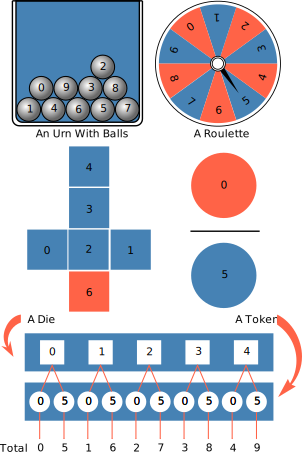
\includegraphics[width=0.82\textwidth]{figures/random-generators.pdf}
\caption{Three types of random number generators: urns, dice and roulettes.
\label{random-generators}}
 \end{figure}
%\clearpage
\txthead{Tables of Random Numbers.} An example of a random number table is
shown in Figure \ref{random-table}. The table consists of three hundred four-digit
numbers. Each digit in the table was chosen randomly, as a result of
a trial, e.g. throwing a die and a token. Therefore, it is understandable
that there is no order in the numbers, and there is no way of predicting
which digit will follow a given one. You could compile many tables after
many trials. Nevertheless, there will not be even the shadow of order in
the sequence of digits.

%\newcolumntype{g}{>{\columncolor{LightYellow}}c}
%\begin{table}[ht]
\begin{figure}[!ht]
\centering
\setlength\arrayrulewidth{1pt}\arrayrulecolor{Tomato}
\renewcommand{\arraystretch}{.9}
\begin{footnotesize}
\begin{tabular}{cccccccccc}
\hline
%&col1 &col2 &col3 &col4 & col5 &col6 &col7\\
%\hline
%\hline
0655 & 8453 & 4467 & 3234 & 5320 & 0709 & 2523 & 9224 & 6271 & 2607 \\
\rowcolor{lightgray}5255 & 5161 & 4889 & 7429 & 4647 & 4331 & 0010 & 8144 & 8638 & 0307 \\
6314 & 8951 & 2335 & 0174 & 6993 & 6157 & 0063 & 6006 & 1736 & 3775 \\
\rowcolor{lightgray} 3157 & 9764 & 4862 & 5848 & 6919 & 3135 & 2837 & 9910 & 7791 & 8941 \\
9052 & 9565 & 4635 & 0653 & 2254 & 5704 & 8865 & 2627 & 7959 & 3682 \\
\hline
4105 & 4105 & 3187 & 4312 & 1596 & 9403 & 6859 & 7802 & 3180 & 4499 \\
\rowcolor{lightgray}1437 & 2851 & 6727 & 5580 & 0368 & 4746 & 0604 & 7956 & 2304 & 8417 \\
4064 & 4171 & 7013 & 4631 & 8288 & 4785 & 6560 & 8851 & 9928 & 2439 \\
\rowcolor{lightgray} 1037 & 5765 & 1562 & 9869 & 0756 & 5761 & 6346 & 5392 & 2986 & 2018 \\
5718 & 8791 & 0754 & 2222 & 2013 & 0830 & 0927 & 0466 & 7526 & 6610 \\
\hline
5127 & 2302 & 1392 & 4413 & 9651 & 8922 & 1023 & 6265 & 7877 & 4733 \\
\rowcolor{lightgray} 9401 & 2423 & 6301 & 2611 & 0650 & 0400 & 5998 & 1863 & 9182 & 9032 \\
4064 & 5228 & 4153 & 2544 & 4125 & 9654 & 6380 & 6650 & 8567 & 5045 \\
\rowcolor{lightgray} 5458 & 1402 & 9849 & 9886 & 5579 & 4171 & 9844 & 0159 & 2260 & 1314 \\
2461 & 3497 & 9785 & 5678 & 4471 & 2873 & 3724 & 8900 & 7852 & 5843 \\
\hline
4320 & 4553 & 2545 & 4436 & 9265 & 6675 & 7989 & 5592 & 3759 & 3431 \\
\rowcolor{lightgray} 3466 & 8269 & 9926 & 7429 & 7516 & 1126 & 6345 & 4576 & 5059 & 7746 \\
9313 & 7489 & 2464 & 2575 & 9284 & 1787 & 2391 & 4245 & 5618 & 0146 \\
\rowcolor{lightgray} 5179 & 8081 & 3361 & 0109 & 7730 & 6256 & 1303 & 6503 & 4081 & 4754 \\
3010 & 5081 & 3300 & 9979 & 1970 & 6279 & 6307 & 7935 & 4977 & 0501 \\
\hline
9599 & 9828 & 8740 & 6666 & 6692 & 5590 & 2455 & 3963 & 6463 & 1609 \\
\rowcolor{lightgray} 4242 & 3961 & 6247 & 4911 & 7264 & 0247 & 0583 & 7679 & 7942 & 2482 \\
3585 & 9123 & 5014 & 6328 & 9659 & 1863 & 0532 & 6313 & 3199 & 7619 \\
\rowcolor{lightgray} 5950 & 3384 & 0276 & 4503 & 3333 & 8967 & 3382 & 3016 & 0639 & 2007 \\
8462 & 3145 & 6582 & 8605 & 7300 & 6298 & 6673 & 6406 & 5951 & 7427 \\
\hline
0456 & 0944 & 3058 & 2545 & 3756 & 2436 & 2408 & 4477 & 5707 & 5441 \\
\rowcolor{lightgray} 0672 & 1281 & 8897 & 5409 & 0653 & 5519 & 9720 & 0111 & 4745 & 7979 \\
5163 & 9690 & 0413 & 3043 & 1014 & 0226 & 5460 & 2835 & 3294 & 3674 \\
\rowcolor{lightgray} 4995 & 9115 & 5273 & 1293 & 7894 & 9050 & 1378 & 2220 & 3756 & 9795 \\
6751 & 6447 & 4991 & 6458 & 9307 & 3371 & 3243 & 2958 & 4738 & 3996 \\
\hline
\end{tabular}
\end{footnotesize}
\caption{A table of random numbers.\label{random-table}}
\end{figure}

This is not amazing. A chance is a chance. But a chance has a reverse
aspect. For instance, try and count how many times each digit occurs in \figr{random-table}. You will find that digit 0 occurs 118 times (the frequency it
appears is $118/1200 = 0.099$), digit 1 occurs 110 times (the frequency it
appears is 0.090), digit 2 occurs 114 times (0.095), digit 3 occurs 125
times (0.104), digit 4 occurs 135 times (0.113), digit 5 occurs 135 times
(0.113), digit 6 occurs 132 times (0.110), digit 7 occurs 116 times (0097),
digit 8 occurs 93 times (0.078), and digit 9 occurs 122 times (0.102). We
can see that the appearance frequency for each digit is about the same,
i. e. close to 0.1. Naturally, the reader has come to a conclusion that 0.1
is the \redem{probability} that a digit appears. The reader may say that the
appearance frequency of a digit is close to the probability of its
appearance over a long series of trials (there are 1200 trials here).

Although this is natural, we should wonder once (again how an
unordered set of \redem{random} digits can have an \redem{inherent stability}. This is a demonstration of the reverse aspect of chance and illustrates the
determinism of \redem{probability}.

I advise the reader to ``work'' a little with a random number table (see
\figr{random-table}). For instance, 32 numbers out of the three hundred ones in the table begin with zero, 20 begin with 1, 33 begin with 2, 33 begin with 3,
38 begin with 4, 34 begin with 5, 34 begin with 6, 24 begin with 7, 20
begin with 8, and 32 begin with 9. The probability that a number begins
with a certain digit equals 0.1. It is easy to see that the results of our
count are in a rather good keeping with this probability (one tenth of
three hundred is thirty). However, the deviations are more noticeable
than in the example considered earlier. But this is natural because the
number of trials above was 1200 while here it is much less, only 300.

It is also interesting to count how many times a digit occurs in the
second place (the number of hundreds), in the third place (tens), and the
fourth place (units). It is easy to see that in every case the frequency
with which a given digit appears is close to the probability, i.e. close to
0.1. Thus, zero occurs in the second place 25 times, in the third place 33
times, and in the fourth place 28 times.

An example with the number-plates of motor-cars randomly passing
the observer was cited in the introduction. It was noted that the
probability that the first two digits in the licence number were identical
is 0.1. The probability that the two last digits of the number or two
middle digits or the first and the last digit are identical is the same.



In order to see this, we need not observe a sequence of cars passing
by. We can simply use a random number table (see \figr{random-table}). The four-digit random numbers in the table can be taken as the license numbers
of cars randomly passing the observer. We can see that 40 of the 300
number's have the same two first digits, 28 numbers have the same two
last digits, 24 numbers have the same two middle digits, and 32
numbers have the same first and last digits. In other words, the
frequencies with which a pair of identical digits appears actually
varies around the probability, i.e. in the neighbourhood of 0.1.




\section{Random Events}

When we throw a die or take a ball out of an urn we deal with
a \redem{random event}. There are several interesting problems where the
probability of a random event is required to be found.

\begin{figure}%[!h]
 \centering
 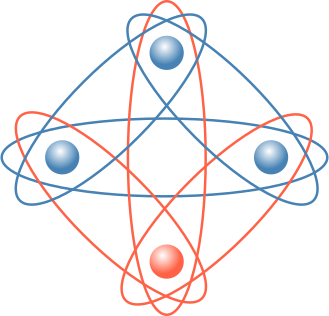
\includegraphics[width=\textwidth]{figures/three-balls.pdf}
\caption{Different ways of taking out two out of three blue and one
  red balls.\label{three-balls}}
\end{figure}


\txthead{A problem with coloured balls.} There are three blue balls and a red
ball in a box. You take two balls out of the box at random. Which is
more probable: that the two balls are blue or that one is blue and one is
red?

People often answer that it is more probable that two blue balls are
taken out because the number of blue balls in the box is three times
greater than the number of red ones. However, the probability of taking
out two blue balls is \redem{equal} to the probability of taking out a blue and
a red ball. You can see this by considering \figr{three-balls}. Clearly there are three ways in which two blue balls may be chosen and three ways of
choosing a blue and a red ball at the same time. Therefore, the
outcomes are equally probable.


We can also calculate the probability of the outcomes. The
probability of taking out two blue balls equals the product of two
probabilities. The first one is the probability of taking out a blue ball
from a set of four balls (three blue ones plus a red one), which is 3/4.
The second probability is that of taking out a blue ball from a set of
three balls (two blue ones plus a red one) which is 2/3. Consequently,
the probability of taking out two blue balls simultaneously is $3/4 \times
2/3 = 1/2$.

The probability of taking out a blue and a red ball is the sum $P_{\text{br}} +
P_{\text{rb}}$, where $P_{\text{br}}$, is the probability of taking out a blue ball from a set of four balls (three blue ones plus a red one) multiplied by the probability of taking out a red ball from a set of three balls (two blue ones plus it red one) and $P_{\text{rb}}$, is the probability of taking out a red ball from a set of four balls (the second all in this case must then be a blue one). In other words, $P_{\text{br}}$ is the probability of taking out a blue ball first and then a red ball while $P_{\text{rb}}$ is the probability of taking out a red ball first and then a blue ball. Inasmuch as $P_{\text{br}} = 3/4 \times 1/3 = 1/4$ and $P_{\text{rb}} = 1/4$, the probability of taking out a pair of differently coloured balls equals $1/4 + 1/4 = 1/2$. 

%\input{figures/fig-10}


\txthead{Throwing A Die: A Game.}  There are two players in this game, player
$A$ and player $B$. The die is thrown three times in succession during each
turn. If a certain face turns up at least once during a turn (let it be a 5),
player $A$ scores a point. But if the five does not turn up, a point is
scored by player $B$. The game is played until one of them scores, say,
a hundred points. Who has the chance of winning greater? Player $A$ or
player $B$?

In order to answer, we first calculate the probability of player
$A$ scoring a point in a turn (the die is thrown three times in succession).
He receives a point in any of the following three cases: if five turns up
in the first trial, if five does not turn up in the first trial but turns up in
the second one, and if five does not turn up in the first two trials but
turns up in the third one. Let us designate the probability of these three
events as $P_{1},  P_{2}$, and $P_{3}$, respectively. The sought probability is $P =
P_{1} + P_{2} + P_{3}$. Note that the probability of five appearing when the die
is thrown is {1/6}, and the probability that five does not appear is {5/6}. It
is clear that $P_{1} = 1/6$. To find $P_{2}$, we should multiply the probability of
the absence of a five in the first trial by the probability of its presence in
the second trial, $P_{2} = 5/6 \times 1/6 = 5/36$. The probability $P_{3}$ is the
product of the probability of the absence of a five in two trials (the first
and the second) and the probability of a five in the third trial, $P_{3}=
(5/6)^{2} \times 1/6 = 25/216$.  Consequently, $ P = P_{1} + P_{2} + P_{3} = 1/6 +
5/6 + 25/216 = 91/216$. Since $P < 1/2$, player $B$ has more chance of
winning this game. We could have reached the same conclusion in
a simpler way by considering the probability of player $B$ scoring a point
after three trials. This is the probability of the absence of five in three
trials: $p = 5/6 \times 5/6 \times 5/6 = 125/216$. Since $p> 1/2$, player $B$'s chances
are better. Note that $P+p=91/216+125/216=1$. This is natural
because one of the players, $A$ or $B$, must score a point in each turn.

Let us change the rules of the game a little: the die is thrown four
times rather than three times in each turn. The other conditions remain
the same. The probability of player $B$ scoring a point in a turn is
$5/6 \times  5/6 \times 5/6 \times 5/6 =625/1296$. This is less than $1/2$, and therefore now $A$ has a better chance of winning a game.



\txthead{The Problem Of An Astrologer.} A tyrant got angry with an astrologer
and ordered his execution. However, at the last moment the tyrant made
up his mind to give the astrologer a chance to save himself. He took
two black and two white balls and told the astrologer to put them into
two urns at random. The executioner was to choose an urn and pick
a ball out of it at random. If the ball was white, the astrologer would be
pardoned, and if the ball was black, he would be executed. How should
the astrologer distribute the balls between the two urns in order to give
himself the greatest chance of being saved?

\begin{figure}[!ht]
 \centering
 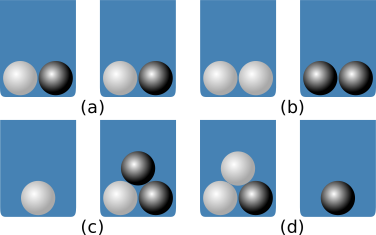
\includegraphics[width=0.75\textwidth]{figures/ball-picking.pdf}
\caption{Different ways of arranging two white and two black balls for
  different probabilities of drawing out a ball of a given colour.\label{ball-picking}}
 \end{figure}

Suppose the astrologer puts a white and a black ball into each urn
(\figr{ball-picking}~\drkgry{(a)}). In this case, no matter which urn the executioner chooses, he will draw a white ball out of it with a probability of 1/2. Therefore, the probability the astrologer would be saved is 1/2.

The probability of the astrologer being saved will be the same if he
puts the two white balls into one urn and the two black balls into the
other (\figr{ball-picking}~\drkgry{(b)}). His destiny will be decided by the executioner when he chooses an urn. The executioner may choose either urn with equal probability.

The best solution for the astrologer is to put a white ball into one um
and a white ball and two black ones into the other urn (\figr{ball-picking}~\drkgry{(c)}). If the executioner chooses the first urn, the astrologer will certainly be saved, but if the executioner picks the second urn, the astrologer will be saved with a probability of {1/3}. Since the executioner chooses either urn with probability {1/2}, the overall probability that the astrologer will be saved is $(1/2 \times 1)+(1/2 \times 1/3)=2/3$.

By contrast, if the astrologer puts a black ball into one urn and
a black ball and two white balls into the other (\figr{ball-picking}~\drkgry{(d)}), the probability of him being saved will be smallest: $(1/2 \times 0)+(1/2 \times 2/3) = 1/3$.

Thus, in order to have the greatest chance of being saved, the
astrologer should distribute the balls between the urns as shown in
(\figr{ball-picking}~\drkgry{(c)}) This is the best strategy. The worst
strategy is to distribute the balls as shown in (\figr{ball-picking}~\drkgry{(d)}). Of course, the selection of the best strategy does not guarantee the desired outcome. Although the risk is decreased, it still remains.

\txthead{Wandering In A Labyrinth.} A labyrinth with treasure has a
death trap, as shown in \figr{labyrinth}. Unlucky treasure-hunters
die in the trap. What is the Probability that they will avoid the trap
and reach the treasure?
\begin{figure}
 \centering
 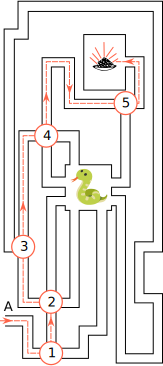
\includegraphics[width=0.9\textwidth]{figures/labyrinth.pdf}
\caption{The probability of finding the treasure or a trap in a labyrinth.\label{labyrinth}}
 \end{figure}
 
After walking away from the entrance $A$ to point {1} (see \figr{labyrinth}) a treasure-hunter may either go straight ahead (in
which case he walks directly into the trap) or turn to the left (in
which case he arrives at point {2}) We shall suppose he picks
either path at random, with equal probability, i.e. with probability
{1/2}. Alter arriving at point {2}, the treasure-hunter may
either go straight ahead or turn right or turn left with probability
{1/3}. The first two paths lead to the trap, while the third path
leads to point {3}. The probability of someone getting from the
entrance $A$ to point {3} is the product of the probability of
turning left at point {1} and the probability of turning left at
point {2}, i.e., $1 /2 \times 1/3$. It is easy to see now that the
probability of reaching point {4} from $A$ is
$1/2 \times 1/3 \times 1/2$; the probability of reaching point {5}
from $A$ is $1/2 \times 1/3 \times 1/2 \times 1/3$; and finally, the
probability of reaching the treasure from $A$ is
$P^{\,+} = 1/2 \times 1/3 \times 1/2 \times 1/3 \times 1/2 = 1/72$. The
only way of getting from the entrance of the labyrinth to the treasure
is shown in the figure by the dash line. The probability that a person
will follow it is thus $P^{\,+} = 1/72$, while the probability of
walking into the trap is $P^{\,-} = 71/72$.




The probability $P^{\,-}$ was calculated from the fact that $P^{\,+} +
P^{\,-} = 1$.  However, we can calculate $P^{\,-}$ directly. Let us expand
$P^{\,-}$ as the sum $P^{\,-} = P_{1} + P_{2} + P_{3} + P_{4} + P_{5}$ where the $P_{i}$ are
  the probabilities of arriving at point $i$ from $A$ multiplied by the
  probability of walking into the trap from point $i \,\, (i = 1, 2, 3, 4,
  5)$.
\begin{align*}
P_{1} & = 1/2, \\
P_{2} &= 1/2 \times 2/3, \\
P_{3} &= 1/2 \times 1/3 \times 1/2,\\
P_{4} &= 1/2 \times  1/3 \times 1/2 \times 2/3,\\
P_{5} & = 1/2 \times 1/3 \times 1/2 \times 1/3 \times 1/2.
\end{align*}
You can then find that $ P_{1} + P_{2} + P_{3} + P_{4} + P_{5} = 71/72$.

\section{Discrete Random Variables}

\txthead{Random Variables.}  Suppose there is a batch of {100}
manufactured articles and {11} articles are rejected as defective, {9}
articles are rejected in another batch of the same size, {10} articles
are rejected in the third one, {12} articles are rejected in the fourth
one, etc. We use $n$ to denote the overall number of manufactured
articles in a batch and $m$ to denote the number of rejected
articles. The number $n$ is constant (here $n = 100$) while the value of $m$
varies from batch to batch in a random manner. Suppose there is a
\redem{definite probability} that there will be $m$ rejected articles in a
randomly selected batch of $n$ articles.  


The number of rejected articles (the variable $m$) is an example of a
\redem{random variable}. \redem{It varies randomly from one trial to
  another, and a certain probability is associated with the occurrence
  of each value of the variable}. Note that we are dealing with a
discrete random variable here, i.e. it may only take a discrete set of
values (the integers from {0} to {100} in this case).

There are also \redem{continuous} random variables. For instance, the
length and weight of newborn babies vary randomly from child to child
and may take any value within a particular interval There are some
special features of continuous random variables which we shall discuss
later; we shall first consider discrete variables.


\txthead{Expected values and variance of a discrete random variable.}
Let $x$ be a discrete random variable which may assume $s$ values: $x_{1}, x_{2},
\ldots x_{m},  \ldots x_{s} $. These values are associated with the probabilities  $p_{1}, p_{2},
\ldots p_{m},  \ldots p_{s} $. For instance, $p_{m}$ is the probability that a variable is $x_{m}$. The sum of all the probabilities $( p_{1} + p_{2} +  \ldots + p_{s})$ is the probability that a trial will give one of the values  $x_{1}, x_{2},  \ldots x_{s} $, (without saying which one). This probability is unity. Consequently,
\begin{equation}%
\sum_{m=1}^{s} \, p_{m}= 1,
\label{eq-1.3}
\end{equation}
\footnote{The notation $\displaystyle \sum_{m=1}^{s}$ means that the summation is performed over all $m$ from 1 to $s$.}
The set of probabilities $p_{1} + p_{2} + \ldots + p_{s}$ (also called
the distribution of the probabilities) contains all the information
needed about the random variable. However, we do not need all the
probabilities for many practical purposes. It is sufficient to know two
most important characteristics of a random variable: its expected
value (its mathematical expectation) and its variance.

The \redem{expected value} is an average value of the random variable taken over a large number of trials. We shall use the letter $E$ to denote the expected value. The expected value of a random variable $x$ is the sum of the products of each variable and its probability, i.e.
\begin{equation*}%
E(x) =  p_{1}x_{1} +  p_{2}x_{2} +  \ldots +  p_{s}x_{s},
\end{equation*}
or using the summation sign,
\begin{equation}%
E(x) = \sum_{m=1}^{s} \, p_{m} \,x_{m}.
\label{eq-1.4}
\end{equation}
We also need to know how a variable deviates from the expected
value, or, in other words, how much the random variable is \redem{scattered}.
The expected value of the deviation from the expected value (that is the
difference $x - E(x)$) cannot be used because it is equal to zero. We can
show this as follows:
\begin{align*}%
E(x- E(x)) & =  \sum_{m=1}^{s} \, p_{m} \, ( x_{m} - E(x)), \\
& =  \sum_{m=1}^{s} \, p_{m} \,x_{m} - E(x) \,  \sum_{m=1}^{s} \,
  p_{m}, \\
& = E(x) - E(x),\\
& = 0.
\end{align*}
This is why the expected value of the \redem{squared} deviation (rather than the expected value of the deviation itself) is used, i.e.
\begin{equation}%
\textrm{var} = \sigma^{2} = E(x — E(x))^{2} = \sum_{m=1}^{s} \, p_{m}
\, ( x_{m} - E(x))^{2}.
\label{eq-1.5}
\end{equation}
This is the variance of a random variable and we shall use var to denote
it. The square root of the variable $\sqrt{\textrm{var}}$ is called the \redem{standard} (or
\redem{root-mean-square) deviation} $\sigma$ of the random variable. It is easy to show that
\begin{equation}
\textrm{var} = E (x^{2}) - (E(x))^{2}. 
\label{eq-1.6}
\end{equation}
Indeed,
\begin{align*}%
 \sum_{m=1}^{s} \, p_{m}  \, ( x_{m} - E(x))^{2} & =  \sum_{m=1}^{s} \, p_{m}
\, ( x_{m}^{2} - 2x_{m} E(x) + E(x))^{2}),\\
& = \sum_{m=1}^{s} \, p_{m}  \,  x_{m}^{2} - 2E(x) \sum_{m=1}^{s} \, p_{m}
\,  x_{m} + (E(x))^{2} \sum_{m=1}^{s} \, p_{m}, \\
& = E(x^{2}) - 2 E(x) E(x) + (E(x))^2,\\
& = E(x^{2}) - (E(x))^{2}.
\end{align*}


\begin{figure}[!h]
 \centering
 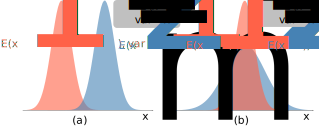
\includegraphics[width=\textwidth]{figures/exp-val-variation.pdf}
\caption{Distributions of random variables with different
  parameters. (a) shows two distributions with different expected
  values but the same variance, while (b) shows two distributions with
  different variance but the same expected values.\label{exp-val-variation}}
 \end{figure}

Two probability distributions are shown in \figr{exp-val-variation}~\drkgry{(a)}. The two random variables possess different expected values while having the same
variance. Looking at \figr{exp-val-variation}~\drkgry{(b)}, we can see a different
picture: the random variables possess different variances while having
the same expected values.


\txthead{Bernoulli's Binomial Distribution.}  Suppose a series of $n$
independent identical trials is performed. The trials are independent
in the sense that the results of any trial do not influence the
results of any other trial. Some trials produce a desired outcome
while the rest do not. Let us call the desired outcome, ``event
$U$". This is a random event. Suppose event $U$ occurs in in trials. This
is a random variable. Let us consider the probability $P_{n}\,(m)$ that event
$U$ will occur $m$ times in a series of $n$ trials.


This is a commonly occurring situation. Suppose $n$ manufactured
articles are checked. Then event $U$ is a rejection, and $P_{n}\,(m)$ is
the probability of in articles being rejected out of a set of in
articles Suppose a hospital registers $n$ newborn babies and the event
$U$ is the birth of a girl. Hence $P_{n}\,(m)$ is the probability that
there will be $m$ girls in a set of $n$ newborn babies. Suppose in a
lottery, $n$ tickets are checked, event $U$ is the discovery of a
prize-winning ticket, and $P_{n}\,(m)$ is the probability that $m$
prize-winning tickets will be found out of a total of $n$
tickets. Suppose in a physics experiment $n$ neutrons are recorded,
the event $U$ is the occurrence of a neutron with an energy within a
certain range, and $P_{n}\,(m)$ is the probability that $m$ of the $n$
neutrons will possess energies in the range. In all these examples,
the probability  $P_{n}\,(m)$ is described by the same formula which is the
\redem{binomial distribution} (sometimes named after a $17^{\text{th}}$ century Swiss mathematician called Jacob Bernoulli).

The binomial distribution is derived by assuming that the probability
that event $U$ will occur in a single trial is known and does not vary
from trial to trial. Let us call this probability $p$. The probability that
event $U$ does not occur in a single trial is $q= 1 - p$. It is important that
the probability that an article is rejected does not depend in any way on
how many rejected articles there are in the given batch. The probability
that a girl is born in any actual delivery does not depend on whether
a girl or a boy was born in the previous birth (nor on how many girls
have so far been born). The probability of winning a prize neither
increases nor decreases as the lottery tickets are checked. The
probability that a neutron has an energy in a given range does not
change during the experiment.

Now, \redem{once the probability $p$ that a certain random event will occur in
a single trial is known, we find the probability $P_{n}(m)$ of $m$ occurrences in
a series of $n$ independent identical trials.}

Suppose the event $U$ occurred in the first $m$ trials but did not occur in
$n - m$ trials, then the probability of the situation would be $p^{m}q^{n-m}$.
Naturally, other orders are possible. For instance, event $U$ may not
occur in the first $n - m$ trials and occur in the rest in trials. The
probability of this situation is also $p^{m}q^{n-m}$. There are also other possible situations. There are as many situations as there are ways choosing
$n$ elements taken in at a time (this is written $\begin{psmallmatrix}n \\ m \end{psmallmatrix}$). The probability of each situation is identical and equals  $p^{m}q^{n-m}$. The order in which event $U$ occurs is inessential. It is only essential that it occurs in $m$ trials and does not occur in the remaining $n - m$ trials. The sought probability $P_{n}(m)$ is the sum of the probabilities of each $\begin{psmallmatrix}n \\ m \end{psmallmatrix}$ situation, i.e. the
product of  $p^{m}q^{n-m}$ and $\begin{psmallmatrix}n \\ m \end{psmallmatrix}$:
\begin{equation}%
P_{n}(m) = \mqty(n \\ m) \, p^{m}q^{n-m}.
\label{eq-1.7}
\end{equation}
There is a formula for the number of combinations of $n$ elements taken
$m$ at a time:
\begin{equation}%
\mqty(n \\ m)
= \frac{n!}{m! (n-m)!}
 = \frac{n(n-1)(n-2)\ldots (n-m+1)}{m!}.
\label{eq-1.8}
\end{equation}
Here $n! = 1 \cdot 2 \cdot 3 \cdot \ldots  \cdot n$ (read $n!$ as ``en factorial''), by convention $0 ! = 1$.

Substituting (\ref{eq-1.8}) into (\ref{eq-1.7}), we can find
\begin{equation}%
P_{n}(m) = \frac{n!}{m! (n-m)!} \, p^{m}q^{n-m}.
\label{eq-1.9}
\end{equation}
This is the \redem{binomial distribution}, or the distribution of a binomial
random variable. I shall explain this term below, and we shall see that
\begin{equation}%
\sum_{m=0}^{n}  P_{n}\,(m) = 1.
\label{eq-1.10}
\end{equation}


\begin{figure}[!h]
 \centering
 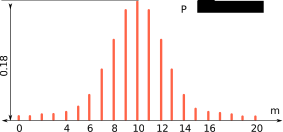
\includegraphics[width=0.8\textwidth]{figures/binomial-dist.pdf}
\caption{The binomial distribution. \label{binomial-dist}}
 \end{figure}


By way of example, let us calculate the probability that $m$ girls are
born in a group of 20 babies. Assume that the probability of delivering
a girl is 1/2, We set $p= 1/2$ and $n = 20$ in expression \eqref{eq-1.9} and consider the integer values of variable $m$ within the range from 0 to 20. The result can be conveniently presented as a diagram (\figr{binomial-dist}). We see that the birth of 10 girls is the most probable; the probability of delivering, for instance, 6 or 14 girls is six times smaller.

If a random variable has a binomial distribution, then its expected
value is
\begin{equation*}
E(m) = \sum_{m=0}^{n} m \, P_{n}(m).
\end{equation*}
or the product of the number of trials and the probability of the event
in a single trial,
\begin{equation}%
E(m) = np.
\label{eq-1.11}
\end{equation}
The variance of such a random variable is the product of the number of
trials, the probability of the occurrence of the event in a single trial, and
the probability it does not occur:
\begin{equation}%
\textrm{var} = E(m^{2}) - (E(m))^2 = npq.
\label{eq-1.12}
\end{equation}


\txthead{The normal (Gaussian) Distribution.} Probability calculations using the
binomial distribution are difficult for large $n$. For instance, in order to
find the probability that 30 girls were delivered from 50 births, you have
to calculate
\begin{equation*}
P_{30}(50) = \frac{50!}{30!20!} (0.5)^{50}.
\end{equation*}
Note that even $20!$ is a 19—digit number. In such cases one can use a
formula which is the limit of the binomial distribution at large $n$:
\begin{equation}%
P_{n}\,(m) = \frac{1}{\sqrt{2 \pi \, \textrm{var}}} \exp \left( -  \frac{(m - E(m))^{2}}{2 \, \textrm{var}}  \right),
\label{eq-1.13}
\end{equation}
where $E\,(m) = np$ and $\textrm{var} = npq$, and $\exp = 2.718 \ldots$
is the base of natural logarithms. The distribution defined in
(\ref{eq-1.13}) is called the \redem{normal} or \redem{Gaussian distribution}.


\txthead{The Poisson Distribution.} If the probability that an event will
occur in a single trial is very small ($p \ll1$), the binomial distribution at
large $n$  becomes the \redem{Poisson} (rather than the normal) distribution, and is defined as
\begin{equation}%
P_{n}\,(m) = \frac{(np)^{m}}{m!} \exp (-np).
\label{eq-1.14}
\end{equation}
This distribution is also sometimes called the \redem{law of rare events}. It is
interesting to note that the variance of a random variable with
the Poisson distribution equals its expected value.

Two distributions are compared in \figr{poisson-gaussian}. The parameters of the
first distribution are $n = 30$ and $p = 0.3$, and it is close to the normal
distribution with the expected value $E\, (m) = 9$. The second distribution’s
parameters are $n = 30$ and $p = 0.05$, and it is close to the Poisson
distribution with $E\,(m)= 1.5$.

\begin{figure}[!h]
 \centering
 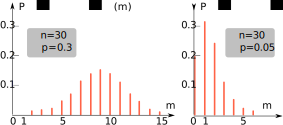
\includegraphics[width=0.9\textwidth]{figures/poisson-gaussian.pdf}
\caption{The Poisson (right) and Gaussian (left) distributions.
\label{poisson-gaussian}}
 \end{figure}

\txthead{A Little of Mathematics.} The expression $(q + p)^{n}$, where $n$ is a positive integer, is called a binomial (two-term) expression of degree $n$. You should know about the binomial expansions of second and third degrees:
\begin{align*}
(q + p)^{2} & = q^{2}+ 2qp + p^{2}, \\
(q + p)^{3} & = q^{3} + 3q^{2}u + 3qp^{2} + p^{3}.
\end{align*}
In general (for a random integer $n$) the binomial expansion is
\begin{equation*}
(q+p)^{n} = q^{n} + nq^{n-1}p + \ldots + \frac{n(n-1) \ldots (n-m+1)}{m!} q^{n-m} p^{m} +
\ldots + nqp^{n-1} + p^{n}.
\end{equation*}
Using the notation given in (\ref{eq-1.8}), we can rewrite this formula as
\begin{equation*}
(q + p)^{n} = \mqty(n \\ 0) \, q^{n}
+  \mqty(n \\ 1)\, q^{n-1}p + \ldots
 +  \mqty(n \\ m) \, q^{n-m}p^{m} + \ldots
+  \mqty(n \\ n-1) \, qp^{n-1} +  \mqty(n \\ n) \, p^{n}.
\end{equation*}
Thus from (\ref{eq-1.9}), we can conclude that
\begin{equation*}
(q + p)^{n} = \sum_{m=0}^{n}  \mqty(n \\ m) \,  q^{n-m}p^{m} = \sum_{m=0}^{n}   P_{n}\,(m).
\end{equation*}
Consequently, the probabilities $P_{n}\, (m)$ coincide with the coefficients of
the binomial expansion, and this is why the \redem{binomial distribution} is so
called. The probabilities $q$ and $p$ in a binomial distribution are such that $q + p = 1$. Therefore, $(q + p)^{n} = 1$. On the other hand,
\begin{equation*}
(q+p)^{n} =  \sum_{m=0}^{n}   P_{n}\,(m).
\end{equation*}
Hence \eqref{eq-1.10}.

\section{Continuous Random Variables}

Continuous random variables are very unlike discrete ones.
A continuous variable can assume any of infinite set of values, which
continuously fill a certain interval. It is impossible in principle to list
every value or such a variable at the very least because there rs no such
thing as two neighbouring values (just as it is impossible to mark two
neighbouring points on the number axis). Besides, the probability of
a concrete value of a continuous random variable is zero.

\txthead{Can Probability Of A Possible Event Equal To Zero?} You know
now that an impossible event has a zero probability. However, a
possible event can also have a zero probability.

Suppose a thin needle is thrown many times at random onto a strip
of paper on which a number axis is marked. We can regard the
$x$-coordinate of the point where the needle crosses the number axis
(\figr{needle}~\drkgry{(a)}) to be a continuous random variable. This coordinate varies in a random fashion from one trial to another.

\begin{figure}[!h]
 \centering
 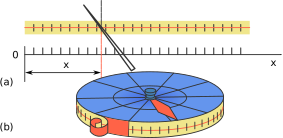
\includegraphics[width=0.8\textwidth]{figures/needle.pdf}
\caption{The probability that a continuous random variable will take a
  certain value is zero.\label{needle}}
 \end{figure}
We could also use a roulette instead of throwing a needle. A strip of
paper with a numbered line could be. pasted to the circumference of
the roulette circle, as shown in \figr{needle}~\drkgry{(b)}. Wherever the freely
rotating arrow of the roulette is pointing when it stops, it yields a
number that will be a continuous random variable.

What is the probability of the arrow stopping at a certain point $x$?
In other words, what is the probability that a concrete value $x$ of a
continuous random variable is chosen? Suppose the roulette
circle's radius $R$ is divided into a finite number of identical
sectors, e.g. 10 sectors (\figr{roulette}). The length of the
arc corresponding to the sector equals $\Delta x = 2 \pi R/10$. The
probability that the arrow will stop within the sector hatched in the
figure is $\Delta x / 2 \pi R = 1/10$. Thus, the probability that the
random variable will take a value from $x$ to $x + \Delta x$ is
$\Delta x / 2 \pi R $. Let us gradually narrow the range of numbers,
i. e. divide the circle into larger numbers of sectors. The
probability $\Delta x / 2 \pi R $ that any value is in the range from
$x$ to $x + \Delta x$ also will fall. In order to obtain the
probability that the variable will take the value $x$ exactly, we must
find the limit as $\Delta x \to 0 $. In this case, the probability
$\Delta x / 2 \pi R $ becomes zero.  Thus we can see that the
probability that a continuous random variable will take a certain
value is indeed zero.

\begin{figure}%[!h]
 \centering
 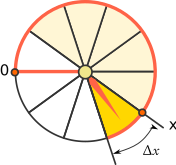
\includegraphics[width=0.9\textwidth]{figures/roulette.pdf}
\caption{A roulette to generate continuous random variables.\label{roulette}}
 \end{figure}

\begin{figure}%[!h]
 \centering
 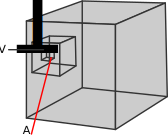
\includegraphics[width=0.9\textwidth]{figures/cubes.pdf}
\caption{A finite non-zero mass can be generated from the sum of an infinite number of zero masses.\label{cubes}}
 \end{figure}


That event may be both possible and possess a zero probability may
seem paradoxical, but it is not. In fact there are parallels you are
surely well aware of. Consider a body of volume $V$ with a mass
$M$. Let us select a point $A$ within the body and consider a smaller
volume $V_{1}$ which contains the point (\figr{cubes}) and
assign a mass $M_{1}$ to it. Let us gradually shrink the smaller
volume around point $A$. We obtain a sequence of volumes containing
$A$, i.e. $V, V_{1}, V_{2}, V_{3}, \ldots ,$ and a corresponding
sequence of decreasing masses: $M, M_{1}, M_{2}, M_{3}, \ldots ,$. The
limit of the mass vanishes as the volume around $A$ contracts to
zero. We can see that a body which has a finite mass consists of
points which have zero masses. In other words, the nonzero mass of the
body is the \redem{sum of an infinite number of zero masses} of its
separate points. In the same way, the nonzero probability that a
roulette arrow stops within a given range $\Delta x$ is the \redem{sum
  of an infinite number of zero probabilities} that the arrow will
stop at each individual value within the considered range.

%\begin{figure}%[!h]
% \centering
% \includegraphics[width=0.4\textwidth]{figures/fig-15.pdf}
%\caption{The nonzero mass of the
%body is the \redem{sum of an infinite number of zero masses} of its
%separate points.}
%\label{fig-1.15}
% \end{figure}




\txthead{The Density Of A Probability.} This conceptual difficulty can
be avoided by using the idea \redem{density}. Although the mass of a
point within a body is zero, the body's density at the point is
non-zero. If $\Delta M$ is the mass of a volume $\Delta V$ within which
the point in question is located (we shall describe the point in terms
of its position vector $\vb{r}$, then the density $\rho \, (\vb{r})$ at
this point is the limit of the ratio $ \Delta M/ \Delta V$ as $\Delta V$ converges to the
point at $\vb{r}$, i.e.,
\begin{equation*}%
\rho \, (\vb{r}) = \lim_{\Delta V \to 0}  \frac{\Delta M}{\Delta V}.
\end{equation*}
If the volume $\Delta V$ is small enough, we can say that $\Delta M
\simeq \rho (\vb{r}) \Delta V$. Using a strict approach, we should
substitute $\Delta V$ by the differential $\dd V$.

The mass $M$ of a body occupying volume $V$ is then expressed by the
\redem{integral}:
\begin{equation*}%
  M = \int_{V} \rho \,  (\vb{r}) \, \dd V,
\end{equation*}
over the volume in question.


Probability theory uses a similar approach. When dealing with
\redem{continuous} random variables, the \redem{probability density} is used rather than the probability itself. Let $f(x)$ be the probability density of a random variable $x$, and so by analogy with the mass density we have
\begin{equation*}%
f(x) = \lim_{\Delta x \to 0 }   \frac{\Delta p_{x}}{\Delta x}.
\end{equation*}
Here $\Delta p_{x}$ is the probability that a random variable will take a value
between $x$ and $x + \Delta x$. The probability $p$ that a random variable will
have a value between $x_{1}$ and $x_{2}$ is, in terms of probability density, as
follows:
\begin{equation}%
p = \int\limits_{x_{1}}^{x_{2}} f(x) \dd x.
\label{eq-1.15}
\end{equation}
If the integration is over the whole range of values a random variable
may take, the integral (\ref{eq-1.15}) will evaluate to unity (this is the probability of a certain event). In the example with a roulette mentioned above,
the whole interval is from $x = 0$ to $x = 2 \pi R$. In general, we assume the
interval is infinite, when 
\begin{equation}%
 \int\limits_{- \infty}^{+ \infty} f(x) dx = 1.
\label{eq-1.16}
\end{equation}
The integral is very simple in the roulette example because the
probability the roulette arrow stops within an interval from $x$ to $x
+ \Delta x$ \redem{does not depend on} $x$. Therefore, the probability
density does not depend on $x$, and hence,


A similar situation is encountered when the density of a body is the
same at every point, i.e. when the body is \redem{uniform} $(\rho = M/V)$. More
generally, density $\rho (\vb{r})$ varies from point to point, and so does the
probability density $f (x)$.


\txthead{The Expected Value And The Variance Of A Continuous Random Variable.} The \redem{expected value} and \redem{variance} of a discrete random
variable are expressed as sums over the probability distribution (see
equations \eqref{eq-1.4} to \eqref{eq-1.6}. When the random variable is
continuous, integrals are used instead of sums and the probability
density distribution is used rather than the probability distribution:
\begin{align}%
E(x) & =  \int\limits_{- \infty}^{+ \infty} x f(x) \, \dd x, 
\label{eq-1.17}\\
\text{var} & =  \int\limits_{- \infty}^{+ \infty} (x - E(x))^{2} f(x) \, \dd x.
\label{eq-1.18}
\end{align}

\txthead{The Normal Distribution Of Probability Density.}
The normal distribution of probability density. When dealing with
continuous random variables, we often encounter the \redem{normal}
distribution of probability density. This distribution is defined by the
following expression (compare it with \eqref{eq-1.13}):
\begin{equation}
f(x) = \frac{1}{\sigma \sqrt{2 \pi}} \exp \left( - \frac{(x - E(x))^2}{2 \sigma ^{2}}\right).
\label{eq-1.19}
\end{equation}

Here $\sigma$ is the standard deviation ($\sigma = \sqrt{var}$) the
function \eqref{eq-1.19} is called the \redem{normal} or \redem{Gaussian
  distribution}.

The probability density of a continuous random variable is always
normal if the variance of its values is due to many different equally
strong factors. It has been proved in probability theory that the sum of
a large enough number of independent random variables obeying any
distributions tends to the normal distribution, and the larger the number
of sums the more accurately the normal distribution is.



For instance, suppose we are dealing with the production of nuts and
bolts. The scatter of the inside diameter of the nut is due to random
deviations in the properties of the metal, the temperature, vibration of
the machine tool, changes in the voltage, wear of the cutter, etc. All of
these effects act independently and approximately with the same
strength. They are superimposed, and the result is that the inside
diameter of the nuts is a continuous random variable with a normal
distribution. The expected value of this variable should evidently be the
desired inside diameter of the nuts, while the variance characterizes the
scatter of the obtained diameters around the desired value.


\begin{figure}[!ht]
 \centering
 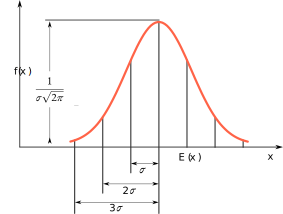
\includegraphics[width=0.75\textwidth]{figures/three-sigma.pdf}
\caption{The three-sigma rule for a Gaussian distribution.\label{three-sigma}}
 \end{figure}



\txthead{The Three-Sigma Rule.}  A normal distribution is shown in
\figr{three-sigma}. It has a maximum at the expected value $E
(x)$. The curve (the \redem{Gaussian curve}) is bell-shaped and is
symmetric about $E (x)$. The area under the entire curve, i. e. for
the interval $(- \infty < x < + \infty )$, is given by the integral
$ \int_{- \infty}^{+ \infty} f(x) dx$.  Substituting \eqref{eq-1.19}
here, it can be shown that the area is equal to unity. This agrees
with \eqref{eq-1.16}, whose meaning is that the probability of a certain event
is unity. Let us divide the area under the Gaussian curve using
vertical lines (see \figr{three-sigma}). Let us first consider the section
corresponding to the interval  $E (x) -  \sigma  \leq x \leq E(x) + \sigma $. It can be shown (please believe me) that 
\begin{equation*}
\int\limits_{E(x) - \sigma}^{E(x) + \sigma} f(x) dx = 0.683. 
\end{equation*}
This means that the probability of $x$ taking a value in the interval from $E
(x) - \sigma$ to $E (x) + \sigma $ equals 0.683. It can also be calculated that
the probability of $x$ taking a value from $E (x) - 2 \sigma$ to $E
(x) + 2 \sigma $ is 0.954, and the probability of $x$ taking a value in the range of $E (x) - 3 \sigma $ to $E (x) + 3 \sigma $ is 0.997. Consequently, a continuous random variable with a normal distribution takes a value in the interval $E (x) - 3 \sigma $ to $ E(x) + 3 \sigma $ with probability 0.997. This probability is practically equal to unity. Therefore, it is natural to assume for
all practical purposes that a random variable will always take a value in the interval from $3 \sigma$ on the right to $3 \sigma$ on the left of $E (x)$. This is called the \redem{three-sigma rule}.
%%% Local Variables:
%%% mode: latex
%%% TeX-engine: xetex
%%% TeX-master: "twibop2"
%%% End:
